\documentclass[twoside]{book}

% Packages required by doxygen
\usepackage{fixltx2e}
\usepackage{calc}
\usepackage{doxygen}
\usepackage[export]{adjustbox} % also loads graphicx
\usepackage{graphicx}
\usepackage[utf8]{inputenc}
\usepackage{makeidx}
\usepackage{multicol}
\usepackage{multirow}
\PassOptionsToPackage{warn}{textcomp}
\usepackage{textcomp}
\usepackage[nointegrals]{wasysym}
\usepackage[table]{xcolor}

% Font selection
\usepackage[T1]{fontenc}
\usepackage[scaled=.90]{helvet}
\usepackage{courier}
\usepackage{amssymb}
\usepackage{sectsty}
\renewcommand{\familydefault}{\sfdefault}
\allsectionsfont{%
  \fontseries{bc}\selectfont%
  \color{darkgray}%
}
\renewcommand{\DoxyLabelFont}{%
  \fontseries{bc}\selectfont%
  \color{darkgray}%
}
\newcommand{\+}{\discretionary{\mbox{\scriptsize$\hookleftarrow$}}{}{}}

% Page & text layout
\usepackage{geometry}
\geometry{%
  a4paper,%
  top=2.5cm,%
  bottom=2.5cm,%
  left=2.5cm,%
  right=2.5cm%
}
\tolerance=750
\hfuzz=15pt
\hbadness=750
\setlength{\emergencystretch}{15pt}
\setlength{\parindent}{0cm}
\setlength{\parskip}{3ex plus 2ex minus 2ex}
\makeatletter
\renewcommand{\paragraph}{%
  \@startsection{paragraph}{4}{0ex}{-1.0ex}{1.0ex}{%
    \normalfont\normalsize\bfseries\SS@parafont%
  }%
}
\renewcommand{\subparagraph}{%
  \@startsection{subparagraph}{5}{0ex}{-1.0ex}{1.0ex}{%
    \normalfont\normalsize\bfseries\SS@subparafont%
  }%
}
\makeatother

% Headers & footers
\usepackage{fancyhdr}
\pagestyle{fancyplain}
\fancyhead[LE]{\fancyplain{}{\bfseries\thepage}}
\fancyhead[CE]{\fancyplain{}{}}
\fancyhead[RE]{\fancyplain{}{\bfseries\leftmark}}
\fancyhead[LO]{\fancyplain{}{\bfseries\rightmark}}
\fancyhead[CO]{\fancyplain{}{}}
\fancyhead[RO]{\fancyplain{}{\bfseries\thepage}}
\fancyfoot[LE]{\fancyplain{}{}}
\fancyfoot[CE]{\fancyplain{}{}}
\fancyfoot[RE]{\fancyplain{}{\bfseries\scriptsize Generated by Doxygen }}
\fancyfoot[LO]{\fancyplain{}{\bfseries\scriptsize Generated by Doxygen }}
\fancyfoot[CO]{\fancyplain{}{}}
\fancyfoot[RO]{\fancyplain{}{}}
\renewcommand{\footrulewidth}{0.4pt}
\renewcommand{\chaptermark}[1]{%
  \markboth{#1}{}%
}
\renewcommand{\sectionmark}[1]{%
  \markright{\thesection\ #1}%
}

% Indices & bibliography
\usepackage{natbib}
\usepackage[titles]{tocloft}
\setcounter{tocdepth}{3}
\setcounter{secnumdepth}{5}
\makeindex

% Hyperlinks (required, but should be loaded last)
\usepackage{ifpdf}
\ifpdf
  \usepackage[pdftex,pagebackref=true]{hyperref}
\else
  \usepackage[ps2pdf,pagebackref=true]{hyperref}
\fi
\hypersetup{%
  colorlinks=true,%
  linkcolor=blue,%
  citecolor=blue,%
  unicode%
}

% Custom commands
\newcommand{\clearemptydoublepage}{%
  \newpage{\pagestyle{empty}\cleardoublepage}%
}

\usepackage{caption}
\captionsetup{labelsep=space,justification=centering,font={bf},singlelinecheck=off,skip=4pt,position=top}

%===== C O N T E N T S =====

\begin{document}

% Titlepage & ToC
\hypersetup{pageanchor=false,
             bookmarksnumbered=true,
             pdfencoding=unicode
            }
\pagenumbering{alph}
\begin{titlepage}
\vspace*{7cm}
\begin{center}%
{\Large Unity Spline Editor }\\
\vspace*{1cm}
{\large Generated by Doxygen 1.8.14}\\
\end{center}
\end{titlepage}
\clearemptydoublepage
\pagenumbering{roman}
\tableofcontents
\clearemptydoublepage
\pagenumbering{arabic}
\hypersetup{pageanchor=true}

%--- Begin generated contents ---
\chapter{Hierarchical Index}
\section{Class Hierarchy}
This inheritance list is sorted roughly, but not completely, alphabetically\+:\begin{DoxyCompactList}
\item \contentsline{section}{Curve\+Point}{\pageref{class_curve_point}}{}
\item Editor\begin{DoxyCompactList}
\item \contentsline{section}{Spline\+Editor}{\pageref{class_spline_editor}}{}
\end{DoxyCompactList}
\item Mono\+Behaviour\begin{DoxyCompactList}
\item \contentsline{section}{Spline\+Creator}{\pageref{class_spline_creator}}{}
\item \contentsline{section}{Spline\+Follow}{\pageref{class_spline_follow}}{}
\end{DoxyCompactList}
\item \contentsline{section}{Spline}{\pageref{class_spline}}{}
\end{DoxyCompactList}

\chapter{Class Index}
\section{Class List}
Here are the classes, structs, unions and interfaces with brief descriptions\+:\begin{DoxyCompactList}
\item\contentsline{section}{\mbox{\hyperlink{class_curve_point}{Curve\+Point}} \\*Represents and anchor point with two control points }{\pageref{class_curve_point}}{}
\item\contentsline{section}{\mbox{\hyperlink{class_spline}{Spline}} \\*This class contains the list of points that make up the spline. Lets you create, get and move those points. }{\pageref{class_spline}}{}
\item\contentsline{section}{\mbox{\hyperlink{class_spline_creator}{Spline\+Creator}} \\*This class will be referenced by the editor script to create and edit splines. }{\pageref{class_spline_creator}}{}
\item\contentsline{section}{\mbox{\hyperlink{class_spline_editor}{Spline\+Editor}} \\*Editor Script that lets us build and draw the spline with a button and add points via mouse click. Updates points\textquotesingle{} positions when they are dragged around. }{\pageref{class_spline_editor}}{}
\item\contentsline{section}{\mbox{\hyperlink{class_spline_follow}{Spline\+Follow}} }{\pageref{class_spline_follow}}{}
\end{DoxyCompactList}

\chapter{Class Documentation}
\hypertarget{class_curve_point}{}\section{Curve\+Point Class Reference}
\label{class_curve_point}\index{Curve\+Point@{Curve\+Point}}


Represents and anchor point with two control points  


\subsection*{Public Member Functions}
\begin{DoxyCompactItemize}
\item 
\mbox{\Hypertarget{class_curve_point_ad10e03f3be123211310318ed71a77962}\label{class_curve_point_ad10e03f3be123211310318ed71a77962}} 
{\bfseries Curve\+Point} (Vector3 anchor\+Pt, Vector3 control\+Pt\+Left, Vector3 control\+Pt\+Right)
\item 
Vector3 \mbox{\hyperlink{class_curve_point_a1d347d73350bdc47a71c17f030507d7f}{Get\+Forward\+Direction}} (Point\+Type type, Transform parent\+Transform=null)
\begin{DoxyCompactList}\small\item\em Gets wherever the control point or anchor is pointing. If a transform is passed, it converts the direction to that transform\textquotesingle{}s local space. \end{DoxyCompactList}\end{DoxyCompactItemize}
\subsection*{Properties}
\begin{DoxyCompactItemize}
\item 
Vector3 \mbox{\hyperlink{class_curve_point_a4770bc5efb8c44892b8216d3a12b645a}{this\mbox{[}\+Point\+Type point\+Type\mbox{]}}}\hspace{0.3cm}{\ttfamily  \mbox{[}get, set\mbox{]}}
\begin{DoxyCompactList}\small\item\em Lets you get one of the three points by type rather than by index \end{DoxyCompactList}\end{DoxyCompactItemize}


\subsection{Detailed Description}
Represents and anchor point with two control points 



\subsection{Member Function Documentation}
\mbox{\Hypertarget{class_curve_point_a1d347d73350bdc47a71c17f030507d7f}\label{class_curve_point_a1d347d73350bdc47a71c17f030507d7f}} 
\index{Curve\+Point@{Curve\+Point}!Get\+Forward\+Direction@{Get\+Forward\+Direction}}
\index{Get\+Forward\+Direction@{Get\+Forward\+Direction}!Curve\+Point@{Curve\+Point}}
\subsubsection{\texorpdfstring{Get\+Forward\+Direction()}{GetForwardDirection()}}
{\footnotesize\ttfamily Vector3 Curve\+Point.\+Get\+Forward\+Direction (\begin{DoxyParamCaption}\item[{Point\+Type}]{type,  }\item[{Transform}]{parent\+Transform = {\ttfamily null} }\end{DoxyParamCaption})}



Gets wherever the control point or anchor is pointing. If a transform is passed, it converts the direction to that transform\textquotesingle{}s local space. 


\begin{DoxyParams}{Parameters}
{\em type} & Anchor, left control or right control point? \\
\hline
\end{DoxyParams}
\begin{DoxyReturn}{Returns}

\end{DoxyReturn}


\subsection{Property Documentation}
\mbox{\Hypertarget{class_curve_point_a4770bc5efb8c44892b8216d3a12b645a}\label{class_curve_point_a4770bc5efb8c44892b8216d3a12b645a}} 
\index{Curve\+Point@{Curve\+Point}!this\mbox{[}\+Point\+Type point\+Type\mbox{]}@{this[Point\+Type point\+Type]}}
\index{this\mbox{[}\+Point\+Type point\+Type\mbox{]}@{this[Point\+Type point\+Type]}!Curve\+Point@{Curve\+Point}}
\subsubsection{\texorpdfstring{this[Point\+Type point\+Type]}{this[PointType pointType]}}
{\footnotesize\ttfamily Vector3 Curve\+Point.\+this\mbox{[}Point\+Type point\+Type\mbox{]}\hspace{0.3cm}{\ttfamily [get]}, {\ttfamily [set]}}



Lets you get one of the three points by type rather than by index 


\begin{DoxyParams}{Parameters}
{\em point\+Type} & The type of the point to get \\
\hline
\end{DoxyParams}
\begin{DoxyReturn}{Returns}

\end{DoxyReturn}


The documentation for this class was generated from the following file\+:\begin{DoxyCompactItemize}
\item 
C\+:/dev/\+Students/\+C\+H15/\+Pamela.\+Figueroa/\+Spline Editor/\+Assets/\+Scripts/\+Spline\+Creation/Curve\+Point.\+cs\end{DoxyCompactItemize}

\hypertarget{class_spline}{}\section{Spline Class Reference}
\label{class_spline}\index{Spline@{Spline}}


This class contains the list of points that make up the spline. Lets you create, get and move those points.  


\subsection*{Public Member Functions}
\begin{DoxyCompactItemize}
\item 
\mbox{\hyperlink{class_spline_ad81797f1f2c52c431f16c75f53370175}{Spline}} (Vector3 anchor\+Pt\+Position, Transform t=null)
\begin{DoxyCompactList}\small\item\em Initializes the point list with two points in a horizontal line. \end{DoxyCompactList}\item 
Vector3 \mbox{\hyperlink{class_spline_a38bbded272df2a9943a90dc33f7c9042}{Get\+Point\+At}} (int index, Point\+Type type, Transform parent\+Transform=null)
\begin{DoxyCompactList}\small\item\em Gets the position of an anchor or control point at a certain index. If a transform is passed, it converts the position into the local space of that transform \end{DoxyCompactList}\item 
\mbox{\Hypertarget{class_spline_a59de318e7ed75528fad1e0e20d476a1a}\label{class_spline_a59de318e7ed75528fad1e0e20d476a1a}} 
\mbox{\hyperlink{class_curve_point}{Curve\+Point}} {\bfseries Get\+Points\+At} (int index)
\item 
void \mbox{\hyperlink{class_spline_a57e6ce88b2b1d1362651dff09b6ef2c8}{Add\+Point}} (Vector3 anchor\+Pt\+Position)
\begin{DoxyCompactList}\small\item\em Add points matching previous anchor point\textquotesingle{}s right handle direction. If we\textquotesingle{}re adding the first point, add control points in a vertial line. \end{DoxyCompactList}\item 
void \mbox{\hyperlink{class_spline_a045ca3ecc4c7e42c054150204833a40c}{Remove\+Point}} (int pointindex)
\begin{DoxyCompactList}\small\item\em Removes anchor point at certain index from list with its control points \end{DoxyCompactList}\item 
void \mbox{\hyperlink{class_spline_ad6d6a6bf25678d717d1f01fcf44fd237}{Add\+Point\+To\+End}} ()
\begin{DoxyCompactList}\small\item\em Add a point to the end of the spline based on the previous point\textquotesingle{}s right handle position. \end{DoxyCompactList}\item 
void \mbox{\hyperlink{class_spline_a3462f1dda107d0ec20ecdff11df7ab88}{Insert\+Point}} (int index)
\begin{DoxyCompactList}\small\item\em Inserts a point after the active point. Grabs the right control point of the previous point and the left one from the next point and puts the new anchor in the middle, with the control points pointing at these. \end{DoxyCompactList}\item 
void \mbox{\hyperlink{class_spline_a33f6df881b5b8980f16bf00fc85034f3}{Set\+Point\+Position}} (int point\+Index, Point\+Type point\+Type, Vector3 new\+Positiion)
\begin{DoxyCompactList}\small\item\em Change position of a certain point.\+When moving points, it makes sure that control points move with the anchor point and that they always form a tangent \end{DoxyCompactList}\item 
Vector3 \mbox{\hyperlink{class_spline_a2fe054cea6de6ba365d29a15ff37696e}{Get\+Position\+For\+Time}} (float time, Transform parent\+Transform)
\begin{DoxyCompactList}\small\item\em Calculate the segment we\textquotesingle{}re at and the position for the provided time. \end{DoxyCompactList}\item 
Vector3 \mbox{\hyperlink{class_spline_ad64325ef2a69decba37df63869d994e9}{Get\+First\+Derivative}} (Vector3 first\+Anchor, Vector3 right\+Control, Vector3 left\+Control, Vector3 second\+Anchor, float t)
\begin{DoxyCompactList}\small\item\em Get first derivative of the points of a segment to get tangent at a certain point in time \end{DoxyCompactList}\item 
Vector3 \mbox{\hyperlink{class_spline_a4dd656d9e96338baa6225ed4d781a943}{Get\+Velocity\+For\+Time}} (float time, Transform parent\+Transform)
\begin{DoxyCompactList}\small\item\em Calculate segment we\textquotesingle{}re at and get tangent for the provided time \end{DoxyCompactList}\item 
Vector3 \mbox{\hyperlink{class_spline_a6747581a7cb4cc9f59eaa751c326c909}{Get\+Direction\+For\+Time}} (float time, Transform parent\+Transform)
\begin{DoxyCompactList}\small\item\em Normalize the velocity vector to get a direction \end{DoxyCompactList}\end{DoxyCompactItemize}
\subsection*{Public Attributes}
\begin{DoxyCompactItemize}
\item 
\mbox{\Hypertarget{class_spline_ac360272353e20dcba514dd78b9798287}\label{class_spline_ac360272353e20dcba514dd78b9798287}} 
bool {\bfseries is\+Looping} = false
\end{DoxyCompactItemize}
\subsection*{Properties}
\begin{DoxyCompactItemize}
\item 
\mbox{\Hypertarget{class_spline_a1f1c156071dde8fb73aa30e2f6abe921}\label{class_spline_a1f1c156071dde8fb73aa30e2f6abe921}} 
int {\bfseries Total\+Segments}\hspace{0.3cm}{\ttfamily  \mbox{[}get\mbox{]}}
\item 
\mbox{\Hypertarget{class_spline_a4ff4ecc0ff40ee96b125dc25789b420f}\label{class_spline_a4ff4ecc0ff40ee96b125dc25789b420f}} 
int {\bfseries Total\+Points}\hspace{0.3cm}{\ttfamily  \mbox{[}get\mbox{]}}
\end{DoxyCompactItemize}


\subsection{Detailed Description}
This class contains the list of points that make up the spline. Lets you create, get and move those points. 



\subsection{Constructor \& Destructor Documentation}
\mbox{\Hypertarget{class_spline_ad81797f1f2c52c431f16c75f53370175}\label{class_spline_ad81797f1f2c52c431f16c75f53370175}} 
\index{Spline@{Spline}!Spline@{Spline}}
\index{Spline@{Spline}!Spline@{Spline}}
\subsubsection{\texorpdfstring{Spline()}{Spline()}}
{\footnotesize\ttfamily Spline.\+Spline (\begin{DoxyParamCaption}\item[{Vector3}]{anchor\+Pt\+Position,  }\item[{Transform}]{t = {\ttfamily null} }\end{DoxyParamCaption})}



Initializes the point list with two points in a horizontal line. 


\begin{DoxyParams}{Parameters}
{\em anchor\+Pt\+Position} & The position to create the first point in. \\
\hline
\end{DoxyParams}


\subsection{Member Function Documentation}
\mbox{\Hypertarget{class_spline_a57e6ce88b2b1d1362651dff09b6ef2c8}\label{class_spline_a57e6ce88b2b1d1362651dff09b6ef2c8}} 
\index{Spline@{Spline}!Add\+Point@{Add\+Point}}
\index{Add\+Point@{Add\+Point}!Spline@{Spline}}
\subsubsection{\texorpdfstring{Add\+Point()}{AddPoint()}}
{\footnotesize\ttfamily void Spline.\+Add\+Point (\begin{DoxyParamCaption}\item[{Vector3}]{anchor\+Pt\+Position }\end{DoxyParamCaption})}



Add points matching previous anchor point\textquotesingle{}s right handle direction. If we\textquotesingle{}re adding the first point, add control points in a vertial line. 


\begin{DoxyParams}{Parameters}
{\em anchor\+Pt\+Position} & Position where the anchor point will be added\\
\hline
\end{DoxyParams}
\mbox{\Hypertarget{class_spline_ad6d6a6bf25678d717d1f01fcf44fd237}\label{class_spline_ad6d6a6bf25678d717d1f01fcf44fd237}} 
\index{Spline@{Spline}!Add\+Point\+To\+End@{Add\+Point\+To\+End}}
\index{Add\+Point\+To\+End@{Add\+Point\+To\+End}!Spline@{Spline}}
\subsubsection{\texorpdfstring{Add\+Point\+To\+End()}{AddPointToEnd()}}
{\footnotesize\ttfamily void Spline.\+Add\+Point\+To\+End (\begin{DoxyParamCaption}{ }\end{DoxyParamCaption})}



Add a point to the end of the spline based on the previous point\textquotesingle{}s right handle position. 

\mbox{\Hypertarget{class_spline_a6747581a7cb4cc9f59eaa751c326c909}\label{class_spline_a6747581a7cb4cc9f59eaa751c326c909}} 
\index{Spline@{Spline}!Get\+Direction\+For\+Time@{Get\+Direction\+For\+Time}}
\index{Get\+Direction\+For\+Time@{Get\+Direction\+For\+Time}!Spline@{Spline}}
\subsubsection{\texorpdfstring{Get\+Direction\+For\+Time()}{GetDirectionForTime()}}
{\footnotesize\ttfamily Vector3 Spline.\+Get\+Direction\+For\+Time (\begin{DoxyParamCaption}\item[{float}]{time,  }\item[{Transform}]{parent\+Transform }\end{DoxyParamCaption})}



Normalize the velocity vector to get a direction 


\begin{DoxyParams}{Parameters}
{\em time} & Time for which to get the direction\\
\hline
{\em parent\+Transform} & Convert to this transform\textquotesingle{}s local space \\
\hline
\end{DoxyParams}
\begin{DoxyReturn}{Returns}

\end{DoxyReturn}
\mbox{\Hypertarget{class_spline_ad64325ef2a69decba37df63869d994e9}\label{class_spline_ad64325ef2a69decba37df63869d994e9}} 
\index{Spline@{Spline}!Get\+First\+Derivative@{Get\+First\+Derivative}}
\index{Get\+First\+Derivative@{Get\+First\+Derivative}!Spline@{Spline}}
\subsubsection{\texorpdfstring{Get\+First\+Derivative()}{GetFirstDerivative()}}
{\footnotesize\ttfamily Vector3 Spline.\+Get\+First\+Derivative (\begin{DoxyParamCaption}\item[{Vector3}]{first\+Anchor,  }\item[{Vector3}]{right\+Control,  }\item[{Vector3}]{left\+Control,  }\item[{Vector3}]{second\+Anchor,  }\item[{float}]{t }\end{DoxyParamCaption})}



Get first derivative of the points of a segment to get tangent at a certain point in time 


\begin{DoxyParams}{Parameters}
{\em first\+Anchor} & First anchor of segment\\
\hline
{\em right\+Control} & Right Control Point of First Anchor\\
\hline
{\em left\+Control} & Left Control Point of Second Anchor\\
\hline
{\em second\+Anchor} & Second anchor of segment\\
\hline
{\em t} & \\
\hline
\end{DoxyParams}
\begin{DoxyReturn}{Returns}

\end{DoxyReturn}
\mbox{\Hypertarget{class_spline_a38bbded272df2a9943a90dc33f7c9042}\label{class_spline_a38bbded272df2a9943a90dc33f7c9042}} 
\index{Spline@{Spline}!Get\+Point\+At@{Get\+Point\+At}}
\index{Get\+Point\+At@{Get\+Point\+At}!Spline@{Spline}}
\subsubsection{\texorpdfstring{Get\+Point\+At()}{GetPointAt()}}
{\footnotesize\ttfamily Vector3 Spline.\+Get\+Point\+At (\begin{DoxyParamCaption}\item[{int}]{index,  }\item[{Point\+Type}]{type,  }\item[{Transform}]{parent\+Transform = {\ttfamily null} }\end{DoxyParamCaption})}



Gets the position of an anchor or control point at a certain index. If a transform is passed, it converts the position into the local space of that transform 


\begin{DoxyParams}{Parameters}
{\em index} & Index of the point to fetch \\
\hline
{\em type} & Wether it is an anchor, left control point or right control point \\
\hline
\end{DoxyParams}
\begin{DoxyReturn}{Returns}

\end{DoxyReturn}
\mbox{\Hypertarget{class_spline_a2fe054cea6de6ba365d29a15ff37696e}\label{class_spline_a2fe054cea6de6ba365d29a15ff37696e}} 
\index{Spline@{Spline}!Get\+Position\+For\+Time@{Get\+Position\+For\+Time}}
\index{Get\+Position\+For\+Time@{Get\+Position\+For\+Time}!Spline@{Spline}}
\subsubsection{\texorpdfstring{Get\+Position\+For\+Time()}{GetPositionForTime()}}
{\footnotesize\ttfamily Vector3 Spline.\+Get\+Position\+For\+Time (\begin{DoxyParamCaption}\item[{float}]{time,  }\item[{Transform}]{parent\+Transform }\end{DoxyParamCaption})}



Calculate the segment we\textquotesingle{}re at and the position for the provided time. 


\begin{DoxyParams}{Parameters}
{\em time} & Point in time we want to get the position at \mbox{[}0-\/1\mbox{]}\\
\hline
{\em parent\+Transform} & Convert to this transform\textquotesingle{}s local space\\
\hline
\end{DoxyParams}
\begin{DoxyReturn}{Returns}

\end{DoxyReturn}
\mbox{\Hypertarget{class_spline_a4dd656d9e96338baa6225ed4d781a943}\label{class_spline_a4dd656d9e96338baa6225ed4d781a943}} 
\index{Spline@{Spline}!Get\+Velocity\+For\+Time@{Get\+Velocity\+For\+Time}}
\index{Get\+Velocity\+For\+Time@{Get\+Velocity\+For\+Time}!Spline@{Spline}}
\subsubsection{\texorpdfstring{Get\+Velocity\+For\+Time()}{GetVelocityForTime()}}
{\footnotesize\ttfamily Vector3 Spline.\+Get\+Velocity\+For\+Time (\begin{DoxyParamCaption}\item[{float}]{time,  }\item[{Transform}]{parent\+Transform }\end{DoxyParamCaption})}



Calculate segment we\textquotesingle{}re at and get tangent for the provided time 


\begin{DoxyParams}{Parameters}
{\em time} & Time for which to get the velocity \mbox{[}0-\/1\mbox{]}\\
\hline
{\em parent\+Transform} & Convert to this transform\textquotesingle{}s local space \\
\hline
\end{DoxyParams}
\begin{DoxyReturn}{Returns}

\end{DoxyReturn}
\mbox{\Hypertarget{class_spline_a3462f1dda107d0ec20ecdff11df7ab88}\label{class_spline_a3462f1dda107d0ec20ecdff11df7ab88}} 
\index{Spline@{Spline}!Insert\+Point@{Insert\+Point}}
\index{Insert\+Point@{Insert\+Point}!Spline@{Spline}}
\subsubsection{\texorpdfstring{Insert\+Point()}{InsertPoint()}}
{\footnotesize\ttfamily void Spline.\+Insert\+Point (\begin{DoxyParamCaption}\item[{int}]{index }\end{DoxyParamCaption})}



Inserts a point after the active point. Grabs the right control point of the previous point and the left one from the next point and puts the new anchor in the middle, with the control points pointing at these. 


\begin{DoxyParams}{Parameters}
{\em index} & Index where to insert the new point after\\
\hline
\end{DoxyParams}
\mbox{\Hypertarget{class_spline_a045ca3ecc4c7e42c054150204833a40c}\label{class_spline_a045ca3ecc4c7e42c054150204833a40c}} 
\index{Spline@{Spline}!Remove\+Point@{Remove\+Point}}
\index{Remove\+Point@{Remove\+Point}!Spline@{Spline}}
\subsubsection{\texorpdfstring{Remove\+Point()}{RemovePoint()}}
{\footnotesize\ttfamily void Spline.\+Remove\+Point (\begin{DoxyParamCaption}\item[{int}]{pointindex }\end{DoxyParamCaption})}



Removes anchor point at certain index from list with its control points 


\begin{DoxyParams}{Parameters}
{\em pointindex} & Index of point to remove.\\
\hline
\end{DoxyParams}
\mbox{\Hypertarget{class_spline_a33f6df881b5b8980f16bf00fc85034f3}\label{class_spline_a33f6df881b5b8980f16bf00fc85034f3}} 
\index{Spline@{Spline}!Set\+Point\+Position@{Set\+Point\+Position}}
\index{Set\+Point\+Position@{Set\+Point\+Position}!Spline@{Spline}}
\subsubsection{\texorpdfstring{Set\+Point\+Position()}{SetPointPosition()}}
{\footnotesize\ttfamily void Spline.\+Set\+Point\+Position (\begin{DoxyParamCaption}\item[{int}]{point\+Index,  }\item[{Point\+Type}]{point\+Type,  }\item[{Vector3}]{new\+Positiion }\end{DoxyParamCaption})}



Change position of a certain point.\+When moving points, it makes sure that control points move with the anchor point and that they always form a tangent 


\begin{DoxyItemize}
\item Anchor Point\+: Move control points with it
\item Control Points\+: Move the other control point in the same direction as the one you\textquotesingle{}re moving while keeping the distance. 
\end{DoxyItemize}


\begin{DoxyParams}{Parameters}
{\em point\+Index} & Index of the point to move. \\
\hline
{\em point\+Type} & Anchor, Control Left or Control Right. \\
\hline
{\em new\+Positiion} & Target Position of the point. \\
\hline
\end{DoxyParams}


The documentation for this class was generated from the following file\+:\begin{DoxyCompactItemize}
\item 
C\+:/dev/\+Students/\+C\+H15/\+Pamela.\+Figueroa/\+Spline Editor/\+Assets/\+Scripts/\+Spline\+Creation/Spline.\+cs\end{DoxyCompactItemize}

\hypertarget{class_spline_creator}{}\section{Spline\+Creator Class Reference}
\label{class_spline_creator}\index{Spline\+Creator@{Spline\+Creator}}


This class will be referenced by the editor script to create and edit splines.  


Inheritance diagram for Spline\+Creator\+:\begin{figure}[H]
\begin{center}
\leavevmode
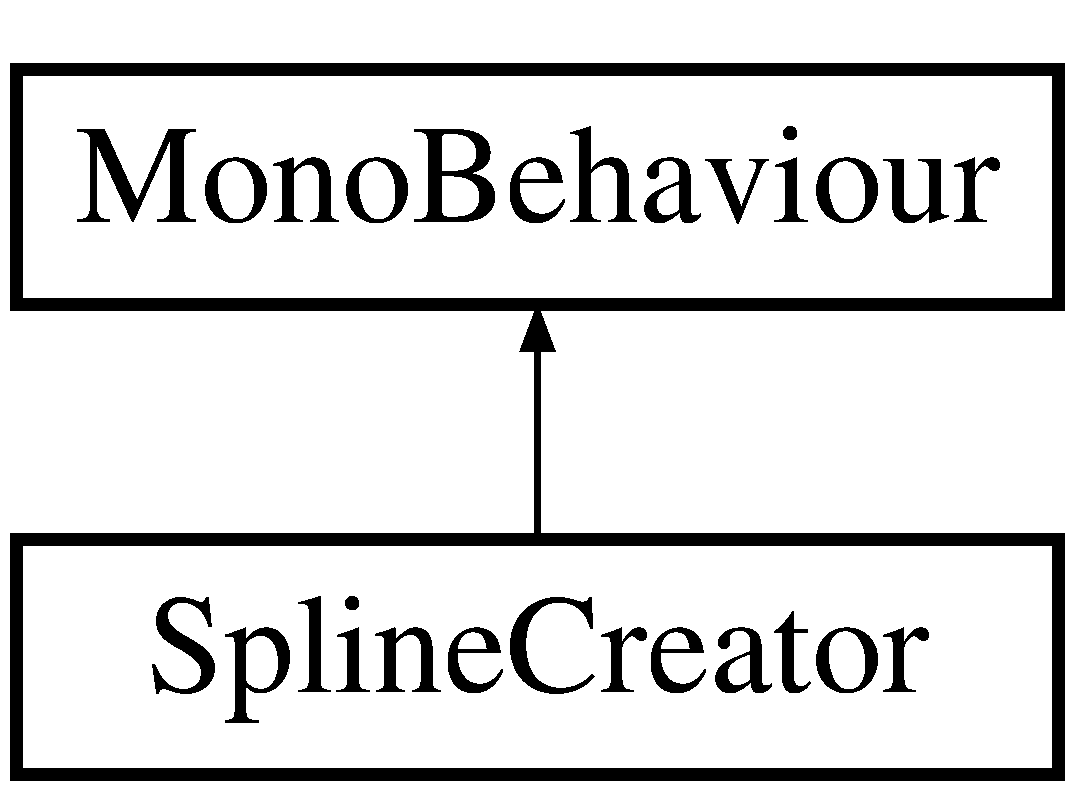
\includegraphics[height=2.000000cm]{class_spline_creator}
\end{center}
\end{figure}
\subsection*{Public Member Functions}
\begin{DoxyCompactItemize}
\item 
\mbox{\Hypertarget{class_spline_creator_a173026c4c682141bff5fc5cac4427524}\label{class_spline_creator_a173026c4c682141bff5fc5cac4427524}} 
void {\bfseries Create\+Spline} ()
\end{DoxyCompactItemize}
\subsection*{Public Attributes}
\begin{DoxyCompactItemize}
\item 
\mbox{\Hypertarget{class_spline_creator_ae619cf1a2abcf7d6c2bef10ff8887215}\label{class_spline_creator_ae619cf1a2abcf7d6c2bef10ff8887215}} 
\mbox{\hyperlink{class_spline}{Spline}} {\bfseries Spline}
\end{DoxyCompactItemize}


\subsection{Detailed Description}
This class will be referenced by the editor script to create and edit splines. 



The documentation for this class was generated from the following file\+:\begin{DoxyCompactItemize}
\item 
C\+:/dev/\+Students/\+C\+H15/\+Pamela.\+Figueroa/\+Spline Editor/\+Assets/\+Scripts/\+Spline\+Creation/Spline\+Creator.\+cs\end{DoxyCompactItemize}

\hypertarget{class_spline_editor}{}\section{Spline\+Editor Class Reference}
\label{class_spline_editor}\index{Spline\+Editor@{Spline\+Editor}}


Editor Script that lets us build and draw the spline with a button and add points via mouse click. Updates points\textquotesingle{} positions when they are dragged around.  


Inheritance diagram for Spline\+Editor\+:\begin{figure}[H]
\begin{center}
\leavevmode
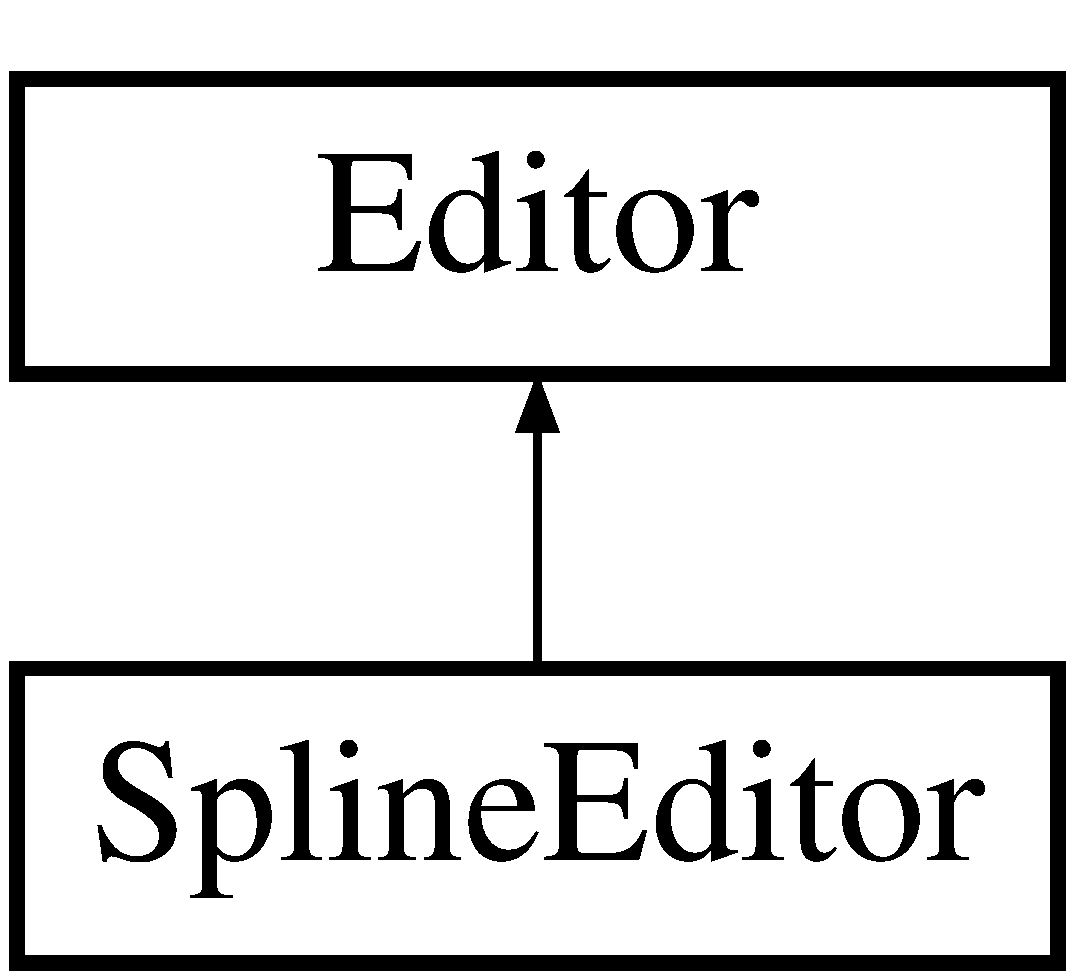
\includegraphics[height=2.000000cm]{class_spline_editor}
\end{center}
\end{figure}
\subsection*{Public Member Functions}
\begin{DoxyCompactItemize}
\item 
\mbox{\Hypertarget{class_spline_editor_af82ef90e17490985629bc79ef10f5795}\label{class_spline_editor_af82ef90e17490985629bc79ef10f5795}} 
override void {\bfseries On\+Inspector\+G\+UI} ()
\end{DoxyCompactItemize}
\subsection*{Public Attributes}
\begin{DoxyCompactItemize}
\item 
\mbox{\Hypertarget{class_spline_editor_a89c507ae57d50b718d38af7e7c3f9918}\label{class_spline_editor_a89c507ae57d50b718d38af7e7c3f9918}} 
float {\bfseries Spline\+Thickness} = 2.\+0f
\end{DoxyCompactItemize}


\subsection{Detailed Description}
Editor Script that lets us build and draw the spline with a button and add points via mouse click. Updates points\textquotesingle{} positions when they are dragged around. 



The documentation for this class was generated from the following file\+:\begin{DoxyCompactItemize}
\item 
C\+:/dev/\+Students/\+C\+H15/\+Pamela.\+Figueroa/\+Spline Editor/\+Assets/\+Scripts/\+Editor/Spline\+Editor.\+cs\end{DoxyCompactItemize}

\hypertarget{class_spline_follow}{}\section{Spline\+Follow Class Reference}
\label{class_spline_follow}\index{Spline\+Follow@{Spline\+Follow}}
Inheritance diagram for Spline\+Follow\+:\begin{figure}[H]
\begin{center}
\leavevmode
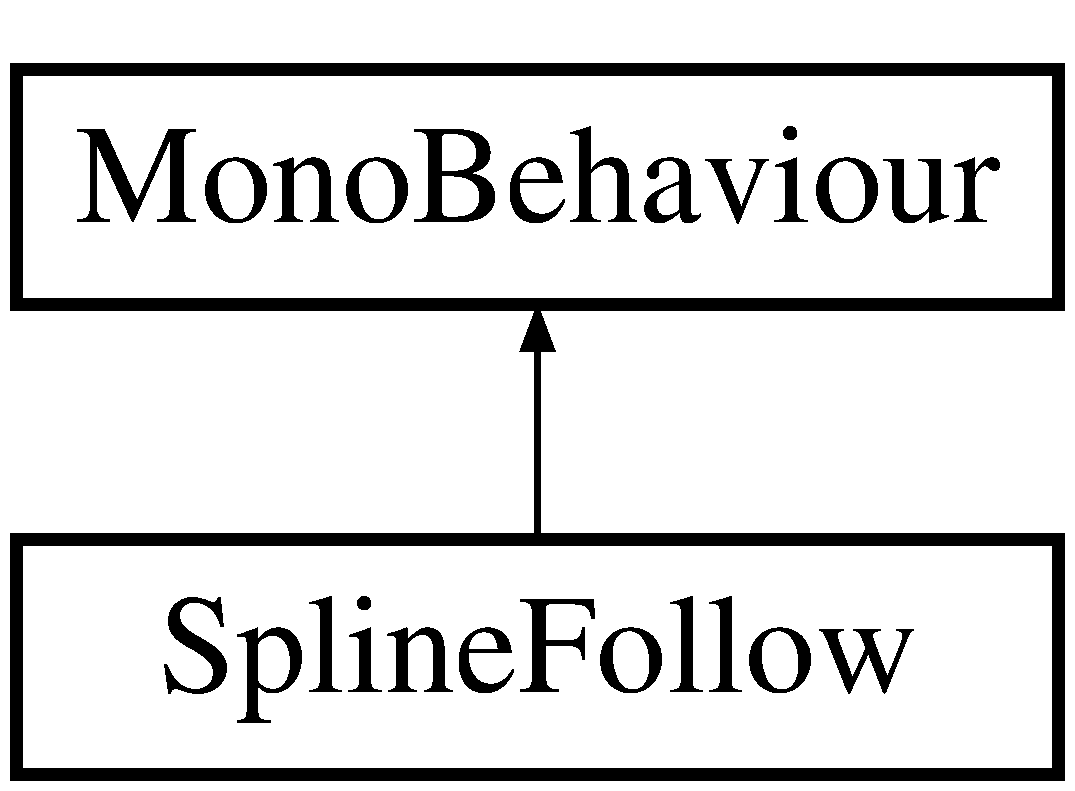
\includegraphics[height=2.000000cm]{class_spline_follow}
\end{center}
\end{figure}
\subsection*{Public Attributes}
\begin{DoxyCompactItemize}
\item 
\mbox{\Hypertarget{class_spline_follow_a6fbb7307ac86b91f19a3c1f82055a14b}\label{class_spline_follow_a6fbb7307ac86b91f19a3c1f82055a14b}} 
\mbox{\hyperlink{class_spline_creator}{Spline\+Creator}} {\bfseries Spline\+Creator\+Ref}
\item 
\mbox{\Hypertarget{class_spline_follow_a42a599013c4249e4de2b2e3fcee8cd07}\label{class_spline_follow_a42a599013c4249e4de2b2e3fcee8cd07}} 
float {\bfseries time\+To\+Traverse} = 10f
\end{DoxyCompactItemize}


The documentation for this class was generated from the following file\+:\begin{DoxyCompactItemize}
\item 
C\+:/dev/\+Students/\+C\+H15/\+Pamela.\+Figueroa/\+Spline Editor/\+Assets/\+Scripts/Spline\+Follow.\+cs\end{DoxyCompactItemize}

%--- End generated contents ---

% Index
\backmatter
\newpage
\phantomsection
\clearemptydoublepage
\addcontentsline{toc}{chapter}{Index}
\printindex

\end{document}
